
%%
% \documentclass[nonacm, sigconf, anonymous, review]{acmart}

\documentclass[sigconf, anonymous, review]{acmart}
% \documentclass[sigplan,twocolumn,review,anonymous]{acmart}

%\usepackage{amsmath}
% \usepackage{algorithmic}
%\usepackage{graphicx}
%\usepackage{textcomp}
\usepackage{color}
\usepackage{xcolor}
%\usepackage{booktabs}
\usepackage{algorithm}
%\usepackage{algorithmicx}
%\usepackage{algpseudocode}
%\usepackage{verbatim}
%\usepackage{stfloats}
\usepackage{colortbl}
%\usepackage{amsmath}
%\usepackage{amsthm}
\usepackage{algpseudocode}
%\usepackage{caption}
\usepackage{subcaption}
%\usepackage{url}
\usepackage{multirow}
%\usepackage{hyperref}
%%
%% \BibTeX command to typeset BibTeX logo in the docs
\AtBeginDocument{%
  \providecommand\BibTeX{{%
    Bib\TeX}}}
    
\definecolor{lightgreen}{rgb}{0.85, 0.95, 0.85}
\definecolor{lightpink}{rgb}{1.0, 0.85, 0.85}
\definecolor{mypurple}{rgb}{0.5, 0, 0.5}
\definecolor{myblue}{rgb}{0, 0, 1}

\newcommand{\ynote}[1]{{$\langle${\textcolor{red}{YF: \textbf{#1}}}$\rangle$}}

%% Rights management information.  This information is sent to you
%% when you complete the rights form.  These commands have SAMPLE
%% values in them; it is your responsibility as an author to replace
%% the commands and values with those provided to you when you
%% complete the rights form.
\setcopyright{acmlicensed}
\copyrightyear{2025}
\acmYear{2026}
\acmDOI{XXXXXXX.XXXXXXX}

%% These commands are for a PROCEEDINGS abstract or paper.
\acmConference[Conference acronym 'WWW]{THE ACM WEB CONFERENCE 2026}{June 4--13,
  2026}{Dubai, United Arab Emirates}
%%
%%  Uncomment \acmBooktitle if the title of the proceedings is different
%%  from ``Proceedings of ...''!
%%
%%\acmBooktitle{Woodstock '18: ACM Symposium on Neural Gaze Detection,
%%  June 03--05, 2018, Woodstock, NY}
\acmISBN{978-1-4503-XXXX-X/18/06}


%%
%% Submission ID.
%% Use this when submitting an article to a sponsored event. You'll
%% receive a unique submission ID from the organizers
%% of the event, and this ID should be used as the parameter to this command.
%%\acmSubmissionID{123-A56-BU3}

%%
%% For managing citations, it is recommended to use bibliography
%% files in BibTeX format.
%%
%% You can then either use BibTeX with the ACM-Reference-Format style,
%% or BibLaTeX with the acmnumeric or acmauthoryear sytles, that include
%% support for advanced citation of software artefact from the
%% biblatex-software package, also separately available on CTAN.
%%
%% Look at the sample-*-biblatex.tex files for templates showcasing
%% the biblatex styles.
%%

%%
%% The majority of ACM publications use numbered citations and
%% references.  The command \citestyle{authoryear} switches to the
%% "author year" style.
%%
%% If you are preparing content for an event
%% sponsored by ACM SIGGRAPH, you must use the "author year" style of
%% citations and references.
%% Uncommenting
%% the next command will enable that style.
%%\citestyle{acmauthoryear}


%%
%% end of the preamble, start of the body of the document source.
\begin{document}

%%
%% The "title" command has an optional parameter,
%% allowing the author to define a "short title" to be used in page headers.
\title{From Attack Behavior to Defense Failure: A Stage-Aware Framework for Evaluating APT Defense Capability}

%%
%% The "author" command and its associated commands are used to define
%% the authors and their affiliations.
%% Of note is the shared affiliation of the first two authors, and the
%% "authornote" and "authornotemark" commands
%% used to denote shared contribution to the research.
\author{Ben Trovato}
\authornote{Both authors contributed equally to this research.}
\email{trovato@corporation.com}
\orcid{1234-5678-9012}
\author{G.K.M. Tobin}
\authornotemark[1]
\email{webmaster@marysville-ohio.com}
\affiliation{%
  \institution{Institute for Clarity in Documentation}
  \city{Dublin}
  \state{Ohio}
  \country{USA}
}

\author{Lars Th{\o}rv{\"a}ld}
\affiliation{%
  \institution{The Th{\o}rv{\"a}ld Group}
  \city{Hekla}
  \country{Iceland}}
\email{larst@affiliation.org}

\author{Valerie B\'eranger}
\affiliation{%
  \institution{Inria Paris-Rocquencourt}
  \city{Rocquencourt}
  \country{France}
}

\author{Aparna Patel}
\affiliation{%
 \institution{Rajiv Gandhi University}
 \city{Doimukh}
 \state{Arunachal Pradesh}
 \country{India}}

\author{Huifen Chan}
\affiliation{%
  \institution{Tsinghua University}
  \city{Haidian Qu}
  \state{Beijing Shi}
  \country{China}}

\author{Charles Palmer}
\affiliation{%
  \institution{Palmer Research Laboratories}
  \city{San Antonio}
  \state{Texas}
  \country{USA}}
\email{cpalmer@prl.com}



%%
%% By default, the full list of authors will be used in the page
%% headers. Often, this list is too long, and will overlap
%% other information printed in the page headers. This command allows
%% the author to define a more concise list
%% of authors' names for this purpose.
\renewcommand{\shortauthors}{Trovato et al.}



\begin{abstract}
Evaluating defenses against Advanced Persistent Threats (APTs) is difficult because existing approaches often measure isolated detections, attack techniques, or product-specific outcomes without preserving how individual defense decisions affect a multi-stage attack campaign. As a result, a high-level detection rate or aggregate score may reveal whether a defense performs well, but provides limited guidance on where the defensive chain failed and what should be repaired.

We present an APT defense evaluation framework that connects playbook-faithful adversary execution with action-level defense observations and repair-oriented scoring. The framework models each attack occurrence as a distinct experimental unit and binds its observed defense outcome to a scoring opportunity representing the first failed victim-side control point. It further incorporates canonical attack phases, defense-technology mappings, and stage-level dependency semantics to aggregate action outcomes into stage, playbook, and overall benchmark scores while preserving a reverse trace from each score to the underlying attack action and control failure.

We construct the benchmark from 53 multi-stage APT playbooks containing 1,796 authoritative raw action occurrences and design an execution protocol that retains the complete action population rather than selecting only representative techniques. Actions that cannot be reproduced natively are explicitly distinguished from exact replay and must preserve attack semantics and defender-relevant telemetry under controlled substitution. The scoring model distinguishes prevention, blocking, detection, and missed actions and supports capability-specific analysis in addition to the overall score.

Our current evaluation executes the benchmark in a controlled networked environment against reproduced defense systems. [FINAL EXPERIMENTAL RESULT SENTENCE: summarize replay coverage, evaluated systems, principal score differences, and one or two repair-oriented findings after the real experiments are complete.] These results are intended to show that APT defense evaluation should measure not only whether attacks are detected, but also where the attack chain remains viable and which defensive control should be strengthened first.
\end{abstract}
%%
%% The code below is generated by the tool at http://dl.acm.org/ccs.cfm.
%% Please copy and paste the code instead of the example below.
%%
\begin{CCSXML}
<ccs2012>
   <concept>
       <concept_id>10010147.10010178.10010219.10010220</concept_id>
       <concept_desc>Computing methodologies~Multi-agent systems</concept_desc>
       <concept_significance>500</concept_significance>
       </concept>
   <concept>
       <concept_id>10011007.10011074</concept_id>
       <concept_desc>Software and its engineering~Software creation and management</concept_desc>
       <concept_significance>300</concept_significance>
       </concept>
 </ccs2012>
\end{CCSXML}

\ccsdesc[500]{Computing methodologies~Multi-agent systems}
\ccsdesc[300]{Software and its engineering~Software creation and management}

%%
%% Keywords. The author(s) should pick words that accurately describe
%% the work being presented. Separate the keywords with commas.
\keywords{Log parsing, LLM, Log analysis}
%% A "teaser" image appears between the author and affiliation
%% information and the body of the document, and typically spans the
%% page.


\received{7 October 2025}
\received[revised]{24 December 2025}
\received[accepted]{13 January 2026}

%%
%% This command processes the author and affiliation and title
%% information and builds the first part of the formatted document.
\maketitle

\section{Introduction}

Advanced Persistent Threat (APT) campaigns unfold as multi-stage operations that may span
days or months before an objective is reached. Recent industry reporting places the global
median dwell time at 14 days in 2025, with cyber-espionage intrusions found considerably
later\cite{mandiant2026mtrends}, attributes a large share of intrusions to credential abuse
and vulnerability exploitation\cite{verizon2025dbir}, and records substantial business
disruption once a breach occurs\cite{ibm2024costdatabreach}. Such figures do not convey the
shape of the defense. Individual actions or stages may have been detected or disrupted even
when the campaign ultimately succeeded, and a campaign that failed may have been stopped by a
single control acting late. Recording only whether a campaign succeeded therefore hides where
defensive capability held and where it was insufficient.

Organizations respond by deploying layered stacks, but deployment is not capability. The
components of such a stack emit evidence with different meanings: one removes a precondition
so that an action cannot be attempted, another interrupts the action while it runs, a third
records it without preventing it, and a fourth does not observe it. Counting products, or
counting alerts, flattens these distinctions. An evaluation useful to a defender must instead
be comparable across heterogeneous stacks, aware of where in a campaign an outcome occurred,
and traceable from an aggregate figure back to a control that can be repaired.

Existing approaches supply parts of this picture. ATT\&CK provides a shared vocabulary for
adversary behavior\cite{mitreAttack} and public product evaluations report responses step by
step\cite{mitreAttackEvaluations}, yet technique coverage has been shown empirically to be a
weak proxy for defensive capability\cite{virkud2024endpoint}. Provenance-based detection and
attack reconstruction recover the causal origin of observed malicious
activity\cite{jiang2025orthrus,goyal2024rcaid}, and control catalogs relate adversary
techniques to countermeasures\cite{mitreCTIDMappings,kaloroumakis2021d3fend}. These outputs
characterize attacker behavior, causal evidence, or candidate countermeasures, but they are
not designed to provide the stable victim-side control attribution required by our
repair-oriented scoring task.

A second line represents how an intrusion advances. Attack graphs and reachability models
reason about attack paths and their
composition\cite{sheyner2002attackgraphs,wang2007measuring}, while severity and system-level
risk models quantify exposure along a different axis\cite{mell2007common,erola2022system};
step-level results have also been re-linked into causal chains to recover campaign
structure\cite{shen2024decoding}. Campaign progress and the control-point domain associated
with an action nevertheless remain orthogonal dimensions: the same control domain can be
implicated at multiple phases, while actions within one phase can map to different control
domains. Collapsing them onto a single axis makes a score harder to act on, not easier.

A third line aggregates observations into an overall figure. Security-metric and
evaluation-validity work reports coverage, detection rates, and paired effectiveness
quantities\cite{iannacone2020quantifiable,zaffarano2015mtd,liu2023defia}, and cautions that
aggregate security numbers are sensitive to how they are
constructed\cite{verendel2009quantified,vanderkouwe2019benchmarkingflaws}. A uniform average
treats action outcomes as interchangeable. Actions within one stage are not: sometimes any
one of them suffices for the attacker, sometimes all are required, and sometimes they form a
loose set. An average cannot represent these alternative, conjunctive, and clustered stage
semantics, and it obscures which actions and stages account for the resulting score loss.

The three limitations above point to a common missing object: an evaluation unit that keeps
attacker behavior, a benchmark-side repair reference, and the evaluated system's response
aligned without conflating them. We therefore pair an in-scope benchmark action with a
reference primary control-point attribution fixed during benchmark construction, and with the
outcome observed when a defense system under test is exercised against that action. The
attribution names one victim-side control point -- a mechanism, configuration, policy, or
operational process -- and is a benchmark-side reference, assigned under a documented
procedure before any system is evaluated. The observed outcome, by contrast, records what the
evaluated system did when the action was exercised. This separation matters because an
attacker-side technique label does not by itself determine a victim-side repair target:
actions sharing the same technique label may require different control-point attributions
depending on their context. Attacker-side and victim-side attribution answer different
questions, and a framework aimed at repair must preserve the second without discarding the
first.

Building an evaluation on this unit raises three methodological challenges. First, the
attribution must remain stable across heterogeneous actions while staying repair-relevant: a
schema too coarse cannot separate distinct repairs, and one too fine cannot be applied
consistently. Second, campaign phase and control-point domain must be carried as separate
dimensions, together with the confidence of each assignment, so that a
downstream figure can be interpreted rather than merely read. Third, action-level outcomes
must be aggregated under the semantics that actually hold inside a stage, and the aggregate
must remain decomposable afterwards.

We address these with a three-step framework. The first step constructs the reference
attribution for benchmark actions, recording a primary control-point reference together with
its confidence under the benchmark schema. Secondary annotations, when present, remain
contextual metadata rather than additional primary scoring targets. The second step enriches
the attributed action into a scoring-ready record, adding the campaign phase at which the
action occurs, the defense product categories expected to address the attributed control
point, and the aggregation semantics governing its stage; phase is carried independently of
the attribution, so that where an action occurs in the campaign remains separate from which
control-point domain it is associated with. The third step aligns observations from a system
under test to benchmark actions, normalizes them onto a common outcome vocabulary of
\texttt{PREVENTED}, \texttt{BLOCKED}, \texttt{DETECTED}, and \texttt{MISSED}, and aggregates
actions to stages and stages to playbooks while retaining breakdowns by phase, control-point
domain, and product category. The current benchmark instance draws on 53 APT playbooks and
1,796 authoritative raw action occurrences; the benchmark presently defines 1,773 active
scoring opportunities, and the control-point schema presently comprises nine top-level domains
and 97 active leaves.

The main contributions of this paper are as follows:
\begin{itemize}
    \item \textbf{An evaluation representation for repair-oriented APT defense scoring.} We
    define the evaluation record so that it extends an attacker-side action description by
    binding to it a reference primary control-point attribution and an observed defense
    outcome, keeping the benchmark-side attribution separate from the behavior of the system
    under test. The attack action remains part of the representation; what the representation
    adds is a repair-oriented victim-side dimension alongside the observed result.

    \item \textbf{A scoring-ready, stage-aware benchmark representation.} We describe a
    construction process that enriches each attributed action with its campaign phase, the
    expected defense product categories, confidence, and explicit stage
    aggregation semantics, keeping campaign progress and victim-side control attribution as
    separate dimensions of one record.

    \item \textbf{A stage-aware aggregation and reporting model.} We separate an action's
    outcome from the weight of the stage containing it, aggregate outcomes under each stage's
    recorded OR, AND, or Cluster semantics rather than a uniform average, compose action to
    stage to playbook scores, and preserve decomposition by action, control point, and phase.
\end{itemize}

% \section{Related Work}
\label{sec:related-work}

Work relevant to this paper answers four questions using four kinds of evidence. \emph{Prospective structural evaluation} asks what an attacker could achieve given a model of configurations, vulnerabilities, and reachability. \emph{Empirical replay observation} asks what a deployed defense did when specific actions were executed against it. \emph{Defense-effectiveness scoring} asks how such results combine into a comparable quantity. \emph{Repair attribution} asks which control should be fixed as a consequence. The four are not interchangeable: a reachable path, an alert, a blocking decision, and a remediation target are different objects, and a score over one cannot be read as a statement about another. We therefore organize prior work by the question it answers and by its unit of analysis.

\subsection{Attack Knowledge Bases, Adversary Emulation, and Defense Benchmark Construction}
\label{subsec:rw-emulation-benchmark}

ATT\&CK supplies the tactic and technique vocabulary used to normalize adversary behavior and derive canonical phases in our benchmark~\cite{mitreAttack}. ATT\&CK Evaluations record how individual products expose or detect procedures during emulation~\cite{mitreAttackEvaluations}, while tooling such as CALDERA~\cite{caldera} makes technique-level tests executable and harnesses such as DELTA orchestrate attacks against a target~\cite{lee2017delta}. These resources yield executable actions and per-product observations, but do not specify how such observations become comparable outcomes, nor how an aggregate points back to a control worth repairing.

Two lines of work evaluate a deployed defense at action granularity by injection or replay, and they are the closest prior art to our evaluation pipeline. SAIBERSOC injects synthetic ATT\&CK-derived attacks into a live security operations center~\cite{rosso2022saibersoc}. Its evaluated object is the operational center as a whole, monitoring infrastructure together with the analysts who staff it; its unit of analysis is an injected attack instance; and it reports detection accuracy separated into identification and investigation, together with time-to-investigation, compared between differently configured centers. Cao et al. replay real-world attack variants against several detection methods and report detection capability per variant~\cite{cao2016replay}; their evaluated object is the detector and their unit is the replayed variant. Both pipelines coincide with ours up to the moment an outcome is recorded. They diverge in what that outcome is designed to explain: SAIBERSOC explains variance attributable to center configuration and analyst process, and Cao et al. explain per-variant detection capability, each appropriate to its own evaluation objective. Our evaluation record instead carries four elements together, the benchmark action, a reference primary control-point attribution fixed before evaluation, the observed defense outcome, and the action's campaign-stage context, so that an aggregate can be decomposed along any of them.

Automated workflows spanning defense generation, enforcement, and evaluation occupy adjacent ground. CD-GEE covers these phases and validates on case-study networks~\cite{enoch2022cdgee}. Its reported evaluation unit is a difference in security posture before and after defense deployment, whereas ours is an outcome observed for a specific evaluated benchmark action. The comparison therefore operates at different granularities: system-level posture in CD-GEE and action-level defense evidence in our framework.

Mappings between controls and attacker behavior are maintained both in research and in industry. D3FEND organizes countermeasures and their relationships to adversary behavior~\cite{mitreD3FEND,kaloroumakis2021d3fend}, prospectively identifying which defensive techniques may be relevant to a behavior, and the MITRE Center for Threat-Informed Defense publishes thousands of technique-to-control mappings with a documented methodology~\cite{mitreCTIDMappings}. Both organize catalogs of defensive controls. Our framework instead uses a victim-side control-point taxonomy and a documented crosswalk between attributed control points and primary or compensating defense categories, and reports agreement statistics for a sampled annotation pilot. Vendor-specific practitioner workflows provide further context: breach-and-attack-simulation and adversarial-exposure-validation products execute attack procedures against a live environment and report control gaps to their operators. We note the practice for its shared concern with observed rather than assumed coverage, and draw no comparison with it, since its methods and results are documented per product.

Our scoring layer consumes observations from systems never designed to be scored. Provenance-based intrusion detection has been systematized as a field~\cite{inam2023sokprovenance}; representatively, HOLMES correlates suspicious flows into campaign-level scenarios~\cite{milajerdi2019holmes} and KAIROS reconstructs compact attack summaries from whole-system provenance~\cite{cheng2024kairos}. On the enforcement side, SANE renders some connectivity architecturally impossible~\cite{casado2006sane}, FIREMAN yields static policy findings~\cite{yuan2006fireman}, and programmable-data-plane defenses interrupt traffic during execution~\cite{zhang2020poseidon,yoo2024smartcookie}. These are representatives of evidence types rather than an inventory: what matters for scoring is the distinction between architectural impossibility, runtime interruption, observation without interruption, and absence of evidence, which map to \texttt{PREVENTED}, \texttt{BLOCKED}, \texttt{DETECTED}, and \texttt{MISSED}.

\subsection{ATT\&CK-Based Coverage and Evaluation Reinterpretation}
\label{subsec:rw-attck-coverage}

A coverage count over ATT\&CK techniques is a tempting capability metric, and it has already been tested. Virkud et al. examine how endpoint detection products and public rulesets use ATT\&CK and show empirically that technique coverage is a poor indicator of defensive capability~\cite{virkud2024endpoint}. Their result is diagnostic, and we build on it rather than re-deriving it. We therefore do not use technique coverage as the score. Evaluation is operationalized one level down, at an attributed action: attributed benchmark actions carry a reference primary control-point attribution, and it is the observed outcome on such an action, rather than the presence of a technique in a coverage list, that enters the score.

Step-level results have also been aggregated across an attack chain. Shen et al. re-link the steps of a published ATT\&CK Evaluations round into causal attack graphs, motivated by the observation that published reports present steps in isolation~\cite{shen2024decoding}. The inputs differ in direction: their evidence is the released output of one existing evaluation, scoped to endpoint products, while ours is a benchmark and attribution layer built from playbooks, which allows a previously unevaluated cross-category defense stack to be scored and its score loss traced to a control.

Both depend on the provenance of the mappings that produce them. Threat-intelligence extraction~\cite{liao2016ioc} and temporal-relation learning over attack steps~\cite{shen2019attack2vec} show such mappings to be derived artifacts, and operational feeds differ substantially in coverage and timeliness~\cite{li2019tealeaves}. We therefore record a confidence label with each attributed action, and the coding guide used during annotation distinguishes how an attribution was reached, rather than treating all mappings as equivalent evidence.

\subsection{Defense Capability and Effectiveness Scoring}
\label{subsec:rw-scoring}

Comparable defense evaluation has been unified before, on a different denominator. Iannacone and Bridges survey the area and express intrusion-detection metrics, cyber-exercise scoring, and security economics through a common cost term~\cite{iannacone2020quantifiable}. Ours is a stage-weighted interception value paired with a repairable control target, so the output is a score that localizes rather than a cost that totals. The cost-oriented lineage is longer still~\cite{butler2002saem,gordon2002economics}, and it illustrates a failure mode we avoid: collapsing incomparable consequences into one index produces a number that is hard to act on, which is why we also report by phase, control-point domain, and product category.

DEFIA is particularly close in intent, scoring the utility of attack behaviors prevented and recording the point at which a defense acts~\cite{liu2023defia}. Its unit of analysis is an attack behavior and its semantics are effectiveness-oriented, resting on whether a behavior was prevented and on where the defense took effect. Three properties of our unit separate the two. Observed outcomes occupy a four-level normalized scale, \texttt{PREVENTED}, \texttt{BLOCKED}, \texttt{DETECTED}, and \texttt{MISSED}, rather than a prevented/not-prevented distinction. Attributed benchmark actions carry a reference primary control-point attribution assigned during benchmark construction, independently of the system under test. And stage membership carries explicit alternative, conjunctive, and clustered composition, which our benchmark must retain when aggregating observed action outcomes from action to stage to playbook.

Prior work on moving-target-defense evaluation already separates complementary views of defense effectiveness. Zaffarano et al. define a quantitative effectiveness framework in which mission-side and attack-side outcomes are measured separately rather than folded into a single figure~\cite{zaffarano2015mtd}, and Taylor et al. apply that framework under automated experimentation, reporting the mission and attack metrics as a pair~\cite{taylor2016mtd}. This separation is the closest structural precedent for our coverage-versus-hit-rate reporting. The evaluated object differs: theirs is a single defense class, moving-target mechanisms, whereas ours is a heterogeneous multi-product stack, so the pairing becomes coverage of the action set structurally applicable to a product category, measured against the hit rate observed within that coverage. Neither work attaches a victim-side control reference to the action or composes outcomes under within-stage semantics. Detection outcomes have likewise been weighted by time: Garcia et al. apply a correcting function per window so that earlier detection scores higher~\cite{garcia2014botnet}. The weighted quantity differs, elapsed detection time in their case and semantic attack phase combined with stage dependency in ours. Time-sensitive and multi-dimensional weighted scoring also appears in live exercises~\cite{doupe2011hitem,werther2011ctf}, where the measured object is a participating team.

Dong et al. assess provenance-based endpoint detection and response tools against operational decision factors such as client overhead and triage cost~\cite{dong2023arewethereyet}. Those dimensions measure the cost of operating a tool; ours characterize observed defense outcomes in campaign context while retaining benchmark-side control-point attribution.

\subsection{Multi-Stage Evaluation, Attack-Path Reasoning, and Repair Prioritization}
\label{subsec:rw-multistage-repair}

Structural methods evaluate multi-stage risk without observing a defense in operation. CVSS scores the severity of an individual vulnerability~\cite{mell2007common,first2019cvss31}, and attack-graph methods reason over configurations, privileges, and reachability through symbolic model checking~\cite{sheyner2002attackgraphs}, logical derivation~\cite{ou2005mulval}, or generation at larger scale~\cite{ou2006scalable}. Derived metrics extend the same view: $k$-zero-day safety counts the unknown vulnerabilities an attacker would require~\cite{wang2014kzero}, network diversity estimates resilience from software heterogeneity~\cite{zhang2016networkdiversity}, and mean time-to-compromise estimates attacker progress across protection zones~\cite{leversage2008mttc}. Each is computed from a model of what is reachable rather than from what a deployed defense did. Attack-graph-based security measurement composes such models into overall metrics for a networked system~\cite{wang2007measuring}, and system-level assessment aggregates risk across an organization's assets~\cite{erola2022system}. These lines organize progression, feasibility, and system-level risk, and they are well suited to those questions. The dimension they organize is nonetheless not the one our attribution supplies: where an action sits in a campaign, and how far an attacker could progress, is a separate question from which class of victim-side control the benchmark associates with that action. We therefore keep campaign phase and control-point domain as independent fields rather than deriving either from the other. Our crosswalk uses structural information in the same prospective spirit, to decide which product categories are expected to cover an action, and reports that applicability separately from empirical performance.

Attack steps have been assigned differentiated defensive value in this setting. GPLADD models multi-step attacker-defender interaction with explicit per-step timing and value~\cite{outkin2019gpladd}, and later work applies the approach to defender policy evaluation and resource allocation using ATT\&CK Evaluations data~\cite{outkin2022defender}. The mode of inference separates the two: that work optimizes allocation probabilistically under uncertainty and outputs a policy, whereas ours computes a deterministic score from observed outcomes and outputs a figure reducible to the attributed actions that account for each score loss.

Repair targets have long been selected from attack models, and this is the prior-work line closest to our attribution contribution. Noel et al. reason over an exploit-dependency graph to identify the initial conditions whose removal makes critical resources unreachable, returning a hardening set rather than a per-event judgement~\cite{noel2003hardening}; Wang, Noel and Jajodia develop the minimum-cost formulation of the same problem, selecting a remediation configuration under cost constraints~\cite{wang2006hardening}. Both operate prospectively over a system and attack model, and both output a set chosen to be sufficient for a reachability goal. The overlap is real: each produces a remediation target from an attack representation. The difference lies in when the target is fixed and what it is attached to. The framework records benchmark-side primary control-point references during benchmark construction, before any system is evaluated, and subsequently aligns observed outcomes to the corresponding benchmark records, aggregating them while action, stage, and control-point traceability is preserved. Unlike minimum-cost hardening, it does not solve for an optimal or sufficient remediation set. Neither output subsumes the other.

The word \emph{attribution} requires disambiguation, because it already denotes a different object in this literature. ORTHRUS defines quality of attribution as the analyst effort needed to recover an attack's causal origin from detection output~\cite{jiang2025orthrus}, and R-CAID embeds root-cause analysis within provenance-based detection~\cite{goyal2024rcaid}. Both reconstruct, explain, or localize attacker-side causal origins in provenance and event space, and both are evaluated on how well that reconstruction succeeds. The attribution in this paper is a different object on a different substrate: a benchmark-side victim-side control-point reference attached to a benchmark action, used for defense scoring and repair-oriented decomposition rather than for explaining an observed intrusion. Neither output subsumes the other, and the shared word should not be read as a shared task.

\begin{table*}[!t]
\centering
\small
\caption{Positioning by evidence, unit of analysis, output, and remediation traceability. Rows group research lines by the question each answers; the grouping does not indicate competitor class.}
\label{tab:related-work-position}
\setlength{\tabcolsep}{3pt}
\begin{tabular}{@{}p{0.155\textwidth}p{0.185\textwidth}p{0.145\textwidth}p{0.190\textwidth}p{0.165\textwidth}@{}}
\hline
\textbf{Research line} & \textbf{Primary evidence} & \textbf{Unit of analysis} & \textbf{Typical output} & \textbf{Remediation traceability} \\
\hline
Knowledge bases, emulation, and replay & Technique descriptions and emulation or replay telemetry & Technique, emulated step, or injected attack & Vocabulary, executable test, or per-attack observation & Partial; process- or capability-oriented \\
ATT\&CK coverage and reinterpretation & Published evaluation outputs and detection rulesets & Technique or evaluation step & Coverage assessment or re-linked attack graph & Indirect; scoped to one product class \\
Effectiveness scoring & Costs, mission metrics, or prevented-behavior utility & Cost-accruing event or attack behavior & Comparable effectiveness or cost index & Aggregate; not tied to one control \\
Multi-stage reasoning and repair prioritization & Configuration, topology, privileges, and modelled paths & Vulnerability, condition, or attack path & Severity, reachability, or minimal hardening set & Structural and prospective \\
Validity and reproducibility & Published benchmarks and evaluation designs & Benchmark, metric, or replication attempt & Methodological constraint or checklist & Not applicable \\
Industry mappings and practitioner validation & Control catalogs and executed attack procedures & Technique--control pair or executed procedure & Mapping set or vendor gap report & Control-oriented; documented per product \\
This work & Playbook action and aligned defense observation & Action--outcome--control record & Stage-aware, multi-dimensional defense score & Explicit reference primary control-point attribution \\
\hline
\end{tabular}
\end{table*}

\subsection{Evaluation Validity, Reproducibility, and Operational Evidence}
\label{subsec:rw-validity}

A unified layer over heterogeneous systems is itself a known construction. Bilot et al. build one for provenance-based intrusion detection, ingesting multiple implementations and reporting comparable metrics~\cite{bilot2025simpler}. The evaluated object differs: detection quality of research prototypes on public datasets in their case, a defense stack evaluated against benchmark playbook actions in our framework, where attributed benchmark records carry a reference primary control-point attribution.

Several results constrain how our scores may be interpreted. Sommer and Paxson argue that designing the evaluation is harder than building the detector~\cite{sommer2010closedworld}, and the base-rate fallacy shows that a low false-positive rate can coexist with a high false-alarm rate under class imbalance~\cite{axelsson2000baserate}, which is why detection denominators must be kept apart. We apply that separation to product-category scoring, reporting coverage over the structurally applicable action set apart from hit rate within it. Verendel finds that quantified-security methods have generally lacked repeated testing~\cite{verendel2009quantified}, and Herley and van Oorschot argue that security claims require explicit assumptions, evidence, and limits of inference~\cite{herley2017science}. We follow these constraints by stating the evidence basis of each reported quantity.

Benchmark validity should be assessed rather than assumed. Van der Kouwe et al. catalog recurring flaws in systems benchmarking and motivate treating benchmark-validity limitations as an explicit subject rather than an implicit one~\cite{vanderkouwe2019benchmarkingflaws}, while Olszewski et al. show that reproduction claims depend on environment and implementation assumptions being made explicit~\cite{olszewski2025replicability}. Both concerns apply to a benchmark of this kind and shape how its reported quantities should be qualified.

One scope limitation follows. The attribution schema covers endpoint, identity, data, network, and operational controls, so a network-based testbed can validate only a replayable slice of the schema rather than its full scope. Actions requiring unsupported endpoint state should be treated as out of scope or as explicit preconditions rather than being assigned a defense outcome.

\subsection{Synthesis and Positioning}
\label{subsec:rw-position}

Table~\ref{tab:related-work-position} summarizes these lines by evidence, unit of analysis, output, and remediation traceability. Existing work separately contributes attacker and action vocabularies together with replay evidence, defense effectiveness and capability metrics, multi-stage and attack-path reasoning, and repair-prioritization or causal-attribution outputs. Each of these components is established, and we claim none of them in isolation. What this framework combines is a benchmark-side reference primary control-point attribution, an observed action outcome on a four-level normalized scale, and explicit within-stage composition semantics, held together so that a comparable defense score remains traceable to the attributed actions and control points that account for it. Simply composing the existing outputs would not achieve this, because an alert, a blocking decision, a posture difference, and a prospective path-risk value do not identify the same evaluated event and cannot be aggregated without an explicit alignment rule. That alignment rule, and the traceability it preserves, is what the action--outcome--control record provides.

\section{Methodology}
\label{sec:methodology}
\begin{figure*}[t]
  \centering
  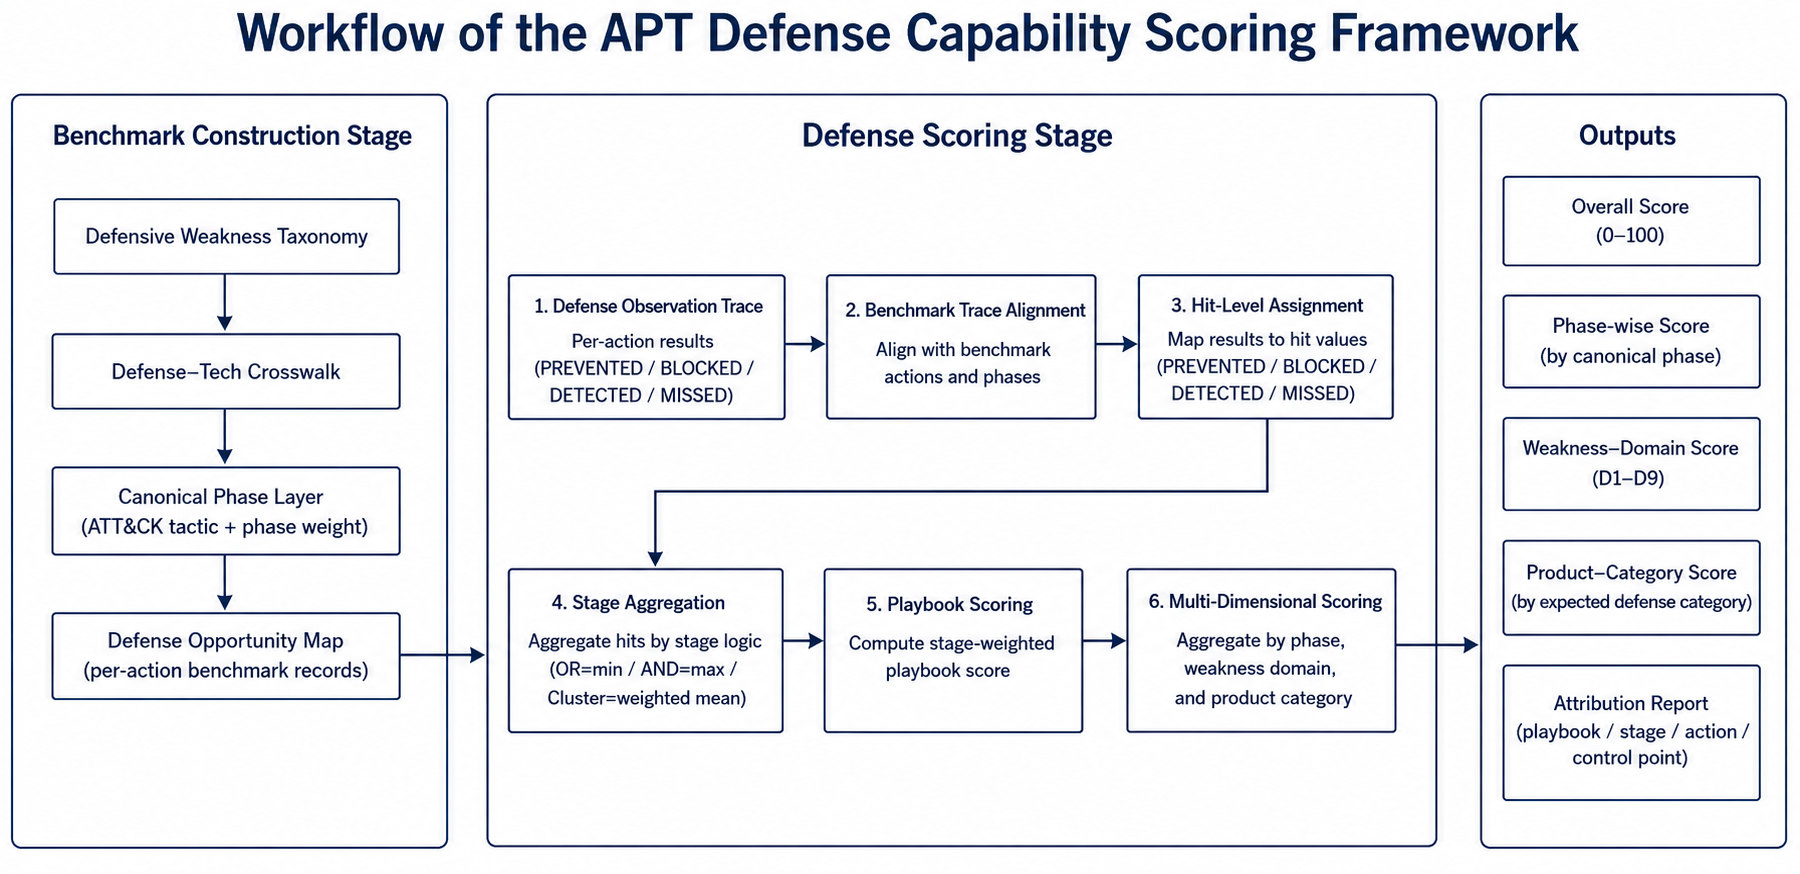
\includegraphics[width=0.95\textwidth]{figs/workflow.png}
  \caption{Workflow of the APT defense capability scoring framework.}
  \Description{Workflow of the proposed APT defense capability scoring framework, including benchmark construction, defense scoring, and score reporting.}
  \label{fig:methodology}
\end{figure*}


\subsection{Overview}
\label{subsec:methodology-overview}

The  framework converts multi-stage APT playbooks and action-level defense observations into interpretable defense capability scores. Its purpose is not only to record whether an attack step was detected or blocked, but also to explain why the step should have been stopped: which victim-side control point first failed, which defense product categories were expected to cover that weakness, and whether the evaluated defenses actually prevented, blocked, or detected the action.

Fig.~\ref{fig:methodology} illustrates the overall workflow. The process has three components: benchmark construction, defense scoring, and score reporting. During benchmark construction, raw APT playbook actions are annotated using a control-point attribution schema. Each action is mapped to the victim-side control point that first failed and is most relevant for repair. The annotated actions are then enriched with canonical attack phases, control-point-to-defense mappings, expected defense product categories, confidence labels, and stage aggregation semantics. The output of this step is a defense opportunity map, where each action is represented as a scoring-ready record.

During defense scoring, the evaluated system provides action-level observation results. Each observation is aligned with its corresponding action record in the defense opportunity map and translated into one of four hit levels: \texttt{PREVENTED}, \texttt{BLOCKED}, \texttt{DETECTED}, or \texttt{MISSED}. These levels capture different degrees of defensive success, from  prevention to complete miss. The scoring engine then aggregates action-level hit values into stage-level and playbook-level scores using the predefined aggregation semantics and canonical phase weights.

The final output is not a single  score. The framework reports an overall defense capability score together with phase scores, control-point domain scores, product category scores, and action level attribution reports. As a result, the score can be traced back to specific playbooks, stages, actions, and failed control points, which directly supports stage aware and attribution driven APT defense evaluation.



\subsection{Defensive Weakness Attribution}
\label{subsec:defensive-weakness-attribution}

We first map each attack action to the victim-side control point that first failed and is most relevant for repair. A control point refers to a defensive mechanism, configuration, policy, or operational process that can be evaluated and remediated independently. In this sense, a successful attack action indicates that a victim-side control was absent, misconfigured, bypassed, or insufficiently enforced.

This scope excludes actions that do not correspond to a directly repairable control point on the victim side. Pre-compromise reconnaissance, attacker-side infrastructure preparation, and similar external prerequisite activities are retained for playbook completeness, but they are not included in primary weakness statistics or attribution-based scoring unless a concrete victim-side control failure can be identified.

This attribution step is necessary because an ATT\&CK label tells us what the attacker did, but it does not tell us which defense failed. The same ATT\&CK technique may be enabled by different weaknesses in different environments. For example, a credential-related action may result from weak password policy, missing multi-factor authentication, exposed remote login services, insufficient credential storage protection, or successful phishing. These cases may share similar attack labels, but they imply different repair actions. Therefore, we interpret each action from the defender's perspective: given this action, which control point should be treated as the primary failure to repair?

Following this view, we use a structured control-point schema to organize recurring victim-side failures. The schema is not organized as an attack sequence. Instead, it separates defensive failures along four design dimensions: security function, architectural location, defensive lifecycle phase, and trust source. Security function distinguishes failures in identity, authorization, execution control, communication protection, and data protection. Architectural location separates externally exposed entry points from internal control failures. Defensive lifecycle phase separates prevention-oriented controls from observability, response, and resilience controls. Trust source captures weaknesses introduced through externally supplied inputs, such as phishing messages, malicious documents, third-party collaboration, and supply-chain entry points.

The schema contains nine top-level control-point domains and 94 fourth-level leaves. The top-level domains provide stable categories for attribution and reporting, while the leaf nodes capture more specific repair targets. In other words, the domains support interpretable scoring, and the leaves provide the operational granularity needed for remediation.

\begin{table}[t]
\centering
\caption{Top-level control-point domains.}
\label{tab:control-point-domains}
\begin{tabular}{p{0.12\columnwidth}p{0.76\columnwidth}}
\hline
Domain & Scope \\
\hline
D1 & Identity, credential, and trust-root failures \\
D2 & Authorization, isolation, and boundary-control failures \\
D3 & Execution, host, and runtime-protection failures \\
D4 & External exposure and remote-entry failures \\
D5 & Communication and protocol-design failures \\
D6 & Data protection, cryptographic-material, and recovery failures \\
D7 & Observability, detection, and response failures \\
D8 & External trust-input failures \\
D9 & Availability and resilience failures \\
\hline
\end{tabular}
\end{table}

Each in-scope action is assigned exactly one primary weakness leaf. This single-label rule keeps later scoring traceable. If a single action had multiple primary attributions, the same failure could be counted several times, and score loss could not be traced to a clear remediation target. To keep attribution consistent, the schema relies on explicit boundary rules and a primary-attribution decision principle: if only one control point could be repaired, the selected leaf should be the one whose repair would most directly prevent or disrupt the action.

Some actions still involve more than one relevant weakness. Secondary weakness tags are used to record such supporting conditions, including dual-control dependencies and entry--root-cause splits. These tags help explain attack chains, but they are not counted as primary attribution results and do not replace the primary leaf used for scoring.

In summary, defensive weakness attribution converts raw attack actions into repair-oriented control-point failures. This attributed action set then becomes the basis for the next steps of the methodology: canonical phase assignment, defense opportunity mapping, and stage-aware scoring.









\subsection{Benchmark Construction}
\label{subsec:benchmark-construction}
After attributing defensive weaknesses, the next step is to convert the attributed playbook actions into benchmark records that can be used for scoring. The attribution result alone is not sufficient for scoring: it tells us which control point failed, but it does not yet specify the attack stage, the expected defense product categories, or the aggregation semantics used later by the scoring engine. Benchmark construction adds these labels without changing the primary attribution result.

The benchmark construction process has three components. First, each action is mapped to a canonical attack phase using ATT\&CK. Second, each control-point leaf is mapped to the defense product categories that are expected to address it. Third, the enhanced action log is written into the defense opportunity map, which will serve as direct input to the scoring phase.

\subsubsection{Canonical Phase Assignment}
The attribution domains describe where the victim-side defense failed, rather than when the action occurs in the attack chain. However, scoring requires stage information because blocking an early-stage action and detecting a late-stage action should not have the same defensive value. Therefore, we add a separate canonical phase layer.

For each action, the framework assigns a canonical phase based on its ATT\&CK technique. We use the ATT\&CK Enterprise tactics as the standard phase vocabulary. Some ATT\&CK techniques can be associated with multiple tactics. We resolve this ambiguity using a predefined technique-to-phase mapping. Each technique is mapped to a single canonical phase before scoring, and this mapping remains fixed during defense scoring. Each technique is mapped to a single canonical phase before scoring, and this mapping remains fixed during defense scoring. Stage-level phases are then derived from the action-level phases, for example by majority voting among the actions in the same playbook stage. This phase assignment is an additional benchmark field; It does not change the control-point attribution described in the previous subsection.

The canonical phase field is later used by the scoring model to apply phase weights. The basic intuition is that earlier interruption has higher defensive value, while late-stage detection provides less benefit because the attacker has already progressed through much of the playbook.

\subsubsection{Defense-Category Mapping}
The primary weakness leaf identifies the failed control point, but a scoring benchmark also needs to know which type of defense product should be expected to address that failure. For this purpose, we build a defense-category mapping between control-point leaves and defense product categories.

Each fourth-level leaf is mapped to two sets of defense categories. The first set is the primary defense category set, which contains product types that should directly prevent or block the corresponding weakness if deployed and configured correctly. The second set is the compensating defense category set, which contains product types that may detect, mitigate, or partially compensate for the weakness, but are not the most direct repair target.

For example, a brute-force action attributed to weak password and anti-brute-force policy is primarily related to identity and access management, while privileged access management or log monitoring may provide compensating support. Similarly, a C2 communication action attributed to missing egress proxy enforcement may be primarily related to network access control or next-generation firewall capabilities, while SIEM or IDS may provide secondary visibility. This mapping allows later scoring to evaluate a product only against the actions that fall within its expected coverage set, rather than applying the same action set to all product categories.

\subsubsection{Defense Opportunity Map}
The final output of benchmark construction is the defense opportunity map. Each record in the map corresponds to one attack action and combines the information needed for scoring: the playbook identifier, stage number, action description, ATT\&CK technique, primary control-point leaf, top-level domain, canonical phase, expected defense categories, confidence label, and stage aggregation semantics.

The opportunity map keeps the primary attribution unique, but it also records additional defense opportunities when they are available. In particular, secondary weakness tags can be expanded into additional leaves and defense categories. This design preserves the repair-oriented primary attribution while still allowing the benchmark to represent layered defense opportunities.


The opportunity map also records the aggregation semantics used for each playbook stage. These semantics specify how the action-level hit values within a stage should be combined during scoring. For example, a stage may represent alternative attack paths, sequentially required actions, or a loose cluster of related actions. The detailed aggregation rules are defined in the scoring model.

Table~\ref{tab:opportunity-record-fields} summarizes the main fields used in the defense opportunity map.

\begin{table}[t]
\centering
\caption{Main fields in a defense opportunity record.}
\label{tab:opportunity-record-fields}
\begin{tabular}{p{0.30\columnwidth}p{0.58\columnwidth}}
\hline
Field & Meaning \\
\hline
playbook, stage, action & Identifier of the attack action in the playbook \\
attack\_id & ATT\&CK technique or sub-technique identifier \\
primary\_leaf & First-failed control-point leaf used for primary attribution \\
primary\_domain & Top-level control-point domain of the primary leaf \\
canonical\_phase & Standard attack phase used for phase-aware scoring \\
primary\_defense & Product categories expected to directly address the weakness \\
compensating\_defense & Product categories that may provide secondary detection or mitigation \\
confidence & Confidence of the primary attribution \\
stage\_logic & Aggregation semantics used later at the stage level \\
\hline
\end{tabular}
\end{table}

Through these steps, benchmark construction turns attributed attack actions into structured defense opportunities. The resulting records connect four pieces of information that are required for scoring: what the attacker did, which victim-side control point first failed, which defense categories were expected to cover the action, and how the action should contribute to stage-level aggregation.


\subsection{Defense Result Alignment}
\label{subsec:defense-result-alignment}
After the benchmark records are constructed, the evaluated defense system provides action-level observation results. Each observation describes how the defense system responded to a specific attack action in the playbook. The purpose of defense result alignment is to match these observations with the corresponding records in the defense opportunity map and convert them into normalized hit values for scoring.

We represent the defense observation trace as a set of action-level records. Each record contains the playbook identifier, the stage number, the action field used in the benchmark, and the observed result. Each defense observation is matched to the action record in the defense opportunity map with the same playbook identifier, stage number, and action field. After alignment, the observed result is associated with the action's control-point attribution, canonical phase, expected defense categories, confidence label, and stage aggregation semantics.

Actions without a matched defense observation are treated as missed actions. Under this rule, an action receives a positive hit value only when the evaluated defense system reports that it was prevented, blocked, or detected. Otherwise, the action is treated as \texttt{MISSED}. It also keeps the benchmark comparable across different defense systems: every system is evaluated against the same set of benchmark actions, and missing observations are interpreted as lack of demonstrated coverage.

Each matched observation is then converted into one of four hit levels. \texttt{PREVENTED} denotes architectural prevention, where the attack path is removed before the action can be attempted. \texttt{BLOCKED} denotes real-time interruption, where the action is attempted but stopped by the defense system. \texttt{DETECTED} denotes successful observation or alerting without stopping the action itself. \texttt{MISSED} denotes the absence of prevention, blocking, or detection. These levels are mapped to numerical hit values used by the scoring model.

\begin{table}[t]
\centering
\caption{Defense observation results and hit values.}
\label{tab:hit-levels}
\begin{tabular}{p{0.24\columnwidth}p{0.14\columnwidth}p{0.50\columnwidth}}
\hline
Result & Hit & Meaning \\
\hline
\texttt{PREVENTED} & 1.0 & The attack path is architecturally removed before the action can occur. \\
\texttt{BLOCKED} & 0.9 & The action is attempted but synchronously interrupted by the defense system. \\
\texttt{DETECTED} & 0.5 & The action is observed or alerted, but not stopped. \\
\texttt{MISSED} & 0.0 & The action is neither prevented, blocked, nor detected. \\
\hline
\end{tabular}
\end{table}

The distinction between \texttt{PREVENTED} and \texttt{BLOCKED} is important. Prevention means that the attack path is unavailable by design, such as when an egress policy makes an unauthorized destination unreachable. Blocking means that the action is observed and interrupted during execution, such as when an endpoint product terminates a malicious process. Both are stronger than detection-only outcomes, but prevention is assigned a slightly higher hit value because it does not depend on runtime recognition of the specific attack instance.

This alignment step produces a unified action-level scoring input. Each benchmark action is associated with both an expected defense opportunity and an observed defense result. 





\subsection{Stage-Aware Scoring Model}
\label{subsec:stage-aware-scoring}
After defense result alignment, each benchmark action has an action-level hit value and a set of benchmark metadata, including its canonical phase, attribution confidence, and stage aggregation semantics. The scoring model uses these fields to compute defense scores at three levels: action, stage, and playbook. The main design principle is to separate defense quality from stage importance. The stage score measures how well the defense performed within a stage, while the stage weight determines how much that stage contributes to the playbook-level score.

Let $a$ denote an attack action. Its hit value $h(a) \in [0,1]$ is obtained from the aligned defense result described in the previous subsection. The action weight $w(a)$ is defined as
\[
w(a) = W_{\mathrm{phase}}(\phi(a)) \cdot C_{\mathrm{conf}}(\gamma(a)),
\]
where $\phi(a)$ is the canonical phase assigned to action $a$, $W_{\mathrm{phase}}$ is the phase-weight function, $\gamma(a)$ is the attribution confidence label, and $C_{\mathrm{conf}}$ is the confidence factor. In our benchmark, the confidence factor reduces the contribution of actions whose attribution is less certain. For example, high-, medium-, and low-confidence actions can be assigned factors of $1.0$, $0.8$, and $0.5$, respectively.

For a playbook stage $s$, let $A_s$ be the set of actions in that stage. The stage score $S_s$ is computed according to the aggregation semantics of the stage. We use three aggregation types: OR, AND, and Cluster.

For an OR stage, the attacker only needs one action in the stage to succeed in order to proceed. Therefore, the defense must block all actions in the stage. The stage score is defined as
\[
S_s = \min_{a \in A_s} h(a).
\]
This reflects the weakest-link constraint: if any action is missed, the stage is considered poorly defended.

For an AND stage, the attacker needs all actions in the stage to succeed in order to complete the stage objective. Therefore, blocking any one required action can disrupt the stage. The stage score is defined as
\[
S_s = \max_{a \in A_s} h(a).
\]
This reflects the strongest defensive interruption within the stage.

For a Cluster stage, the actions do not have a strong logical dependency. They are treated as a group of related behaviors rather than as strict alternatives or strict requirements. The stage score is computed as a weighted average:
\[
S_s =
\frac{\sum_{a \in A_s} h(a) w(a)}
     {\sum_{a \in A_s} w(a)}.
\]
In this case, actions with higher phase importance or higher attribution confidence contribute more to the stage score.

The stage weight is computed separately from the stage score:
\[
W_s = \sum_{a \in A_s} w(a).
\]
This separation avoids mixing the quality of defense within a stage with the importance of that stage in the overall playbook. In particular, OR and AND stage scores are not weighted internally, because their semantics are determined by the attacker's path structure. The weights are used when aggregating stages into a playbook score.

For a playbook $P$ with stages $S(P)$, the playbook-level score is
\[
\mathrm{Score}(P) =
\frac{\sum_{s \in S(P)} W_s S_s}
     {\sum_{s \in S(P)} W_s}.
\]
The overall defense capability score is then computed by aggregating the scores over all evaluated playbooks:
\[
\mathrm{Score}_{\mathrm{overall}} =
\frac{1}{|\mathcal{P}|}
\sum_{P \in \mathcal{P}} \mathrm{Score}(P),
\]
where $\mathcal{P}$ denotes the set of playbooks in the benchmark. This formulation keeps the final score traceable: a score loss can be traced back from the overall score to a playbook, then to a stage, and finally to the individual actions and control-point failures that caused the loss.


\subsection{Multi-Dimensional Score Outputs}
\label{subsec:multi-dimensional-outputs}

The scoring model does not treat the overall score as the only output. A single aggregate score can indicate whether a defense system performs well on average, but does not explain where the score is gained or lost. To support diagnosis and comparison, the framework reports scores from multiple perspectives: overall performance, attack phase, control-point domain, defense product category, and action-level attribution.

The overall score summarizes the performance of the evaluated defense system in all playbooks. It is useful as a compact indicator, but is not intended to be interpreted alone. The same overall score may result from different defense profiles. For example, one system may cover many attack actions but only detect them late, while another system may cover fewer actions but block them reliably within its expected scope. Therefore, the overall score is reported together with the decomposed outputs.

The phase wise score groups results by canonical attack phase. This view answers the question: at which attack phases does the defense system lose the most score? Since the scoring model assigns higher value to earlier interception, phase wise results help distinguish early stage blocking from late stage observation. This directly supports stage aware analysis of APT defense capability.

The control point domain score groups results by the primary victim side control point domain. This view answers a different question: which type of defensive control fails most often or contributes most to score loss? For example, a low score in an identity related domain points to weaknesses in credential and trust controls, while a low score in an observability related domain indicates insufficient detection or response. This decomposition turns an aggregate score into repair-oriented feedback.

The product category score evaluates performance within the expected coverage of each defense product category. For a product category $c$, let $A_c$ denote the set of actions whose defense opportunity records include $c$ as a primary or compensating defense category. The coverage of $c$ is the fraction of benchmark actions that fall into this expected coverage set:
\[
\mathrm{Coverage}(c) = \frac{|A_c|}{|\mathcal{A}|},
\]
where $\mathcal{A}$ is the set of benchmark actions. The hit rate of $c$ is computed only within its coverage set:
\[
\mathrm{HitRate}(c) =
\frac{\sum_{a \in A_c} \tilde{h}_c(a)}
     {|A_c|}.
\]
Here, $\tilde{h}_c(a)$ is the hit value credited to category $c$. Primary defense matches receive full hit credit, while compensating defense matches may receive discounted credit because they detect or mitigate a weakness but do not directly eliminate the failed control point.

Reporting both coverage and hit rate is important. Coverage describes how much of the benchmark a product category is expected to address. Hit rate describes how well it performs within that expected scope. A product with narrow coverage but high hit rate has a different defense profile from a product with broad coverage but low hit rate, even if their aggregate scores are similar.

Finally, the framework produces an action level attribution report. For each score loss, the report retains the playbook, stage, action, ATT\&CK technique, canonical phase, primary control point leaf, defense categories, and observed result. This report provides the trace from aggregate score back to concrete attack actions and failed control points. As a result, the output can support both high level comparison and detailed remediation analysis.

\subsection{Prototype Method Validation}
\label{subsec:prototype-method-validation}

The preceding subsections define the attribution schema, benchmark construction process, result alignment procedure, scoring model, and multi-dimensional outputs. Before applying the framework to real defense-system replay experiments, we perform a set of prototype validation experiments on the benchmark and scoring infrastructure. These experiments do not evaluate a deployed defense product. Instead, they test whether the proposed methodological components are reproducible, whether the control-point--to--defense mapping is reasonable, and whether the scoring engine behaves correctly under boundary and parameter-variation cases.

First, we evaluate the reproducibility of defensive weakness attribution through a pilot inter-rater reliability study. A stratified sample of 50 ATT\&CK techniques and sub-techniques was independently labeled by two annotators using the same coding guide. Agreement was measured at multiple levels, including scope decision, top-level domain, leaf-level attribution, confidence label, mapping method, and secondary weakness tag. Table~\ref{tab:method-irr} summarizes the results.

\begin{table}[t]
\centering
\caption{Prototype validation of defensive weakness attribution.}
\label{tab:method-irr}
\begin{tabular}{p{0.36\columnwidth}p{0.18\columnwidth}p{0.18\columnwidth}p{0.20\columnwidth}}
\hline
Field & Agreement & $\kappa$ & Interpretation \\
\hline
Scope & 100.0\% & 1.000 & Almost perfect \\
L1 domain & 96.0\% & 0.953 & Almost perfect \\
L4 leaf & 86.0\% & 0.856 & Almost perfect \\
Confidence & 82.0\% & 0.679 & Substantial \\
Mapping method & 82.0\% & 0.687 & Substantial \\
Secondary tag & 66.0\% & 0.173 & Slight \\
\hline
\end{tabular}
\end{table}

The result shows that the primary attribution levels are reproducible in the pilot setting. The high agreement at the L1 and L4 levels indicates that the main control-point attribution can be applied consistently. In contrast, the secondary tag has much lower agreement, so it is retained as qualitative chain-context information rather than as a primary quantitative scoring field.

Second, we validate the defense-category mapping used by the Defense--Tech Crosswalk. The external validity check compares the crosswalk categories with the dataset's native control labels. Among 1,733 comparable actions, the two sources agree on 1,297 actions, giving an agreement rate of 74.8\%. We also perform an internal consistency check in which an independent annotator maps a stratified sample of 35 leaves to the 29 defense categories without seeing the existing crosswalk. Table~\ref{tab:method-crosswalk-validation} summarizes these checks.

\begin{table}[t]
\centering
\caption{Prototype validation of defense-category mapping.}
\label{tab:method-crosswalk-validation}
\begin{tabular}{p{0.42\columnwidth}p{0.44\columnwidth}}
\hline
Validation item & Result \\
\hline
External agreement with native control labels & 74.8\% (1,297 / 1,733 actions) \\
Highest category agreement & DLP 96.4\%, NET 93.6\%, EGW 90.3\% \\
Endpoint-category agreement & AV 73.5\%, EDR 71.9\% \\
Primary defense internal agreement & 97.1\% (34 / 35 leaves), $\kappa=0.485$ \\
Compensating defense internal agreement & 45.7\% (16 / 35 leaves), $\kappa=-0.094$ \\
\hline
\end{tabular}
\end{table}

These results suggest that the primary defense mapping is stable enough to support product-category scoring. The lower consistency for compensating defenses indicates that compensating coverage is less sharply defined than primary coverage. Therefore, compensating matches are treated as partial credit and should be interpreted more cautiously.

Third, we check the mathematical behavior of the scoring model using synthetic coverage traces. These traces are not real defense experiments; they are boundary and coverage simulations. A perfect-defense trace assigns \texttt{PREVENTED} to every benchmark action, and a no-defense trace assigns \texttt{MISSED} to every action. Two idealized product-category traces simulate systems that block all actions in their expected EDR or NGFW/NET primary coverage. Table~\ref{tab:method-coverage-simulation} reports the resulting scores.

\begin{table}[t]
\centering
\caption{Prototype scoring checks with synthetic coverage traces.}
\label{tab:method-coverage-simulation}
\begin{tabular}{p{0.26\columnwidth}p{0.52\columnwidth}p{0.12\columnwidth}}
\hline
Simulation & Configuration & Score \\
\hline
Perfect & All actions are \texttt{PREVENTED} & 100.00 \\
None & All actions are \texttt{MISSED} & 0.00 \\
Ideal EDR & EDR primary coverage $\rightarrow$ \texttt{BLOCKED} & 44.40 \\
Ideal NGFW & NGFW/NET primary coverage $\rightarrow$ \texttt{BLOCKED} & 24.93 \\
\hline
\end{tabular}
\end{table}

The perfect and none traces verify the expected upper and lower bounds of the scoring engine. The ideal EDR and ideal NGFW simulations show that a single product category cannot cover the whole benchmark even when it performs perfectly within its expected scope. This result reflects the multi-stage and multi-control nature of APT defense rather than the performance of a specific commercial product.

Finally, we test the robustness of the scoring results under reasonable parameter and aggregation variations. We vary phase weights, confidence factors, and compensating-defense discounts, and we also compare alternative aggregation choices for discovery-heavy Cluster stages and playbook-level aggregation. Table~\ref{tab:method-robustness} summarizes the main results.

\begin{table}[t]
\centering
\caption{Sensitivity and aggregation robustness checks.}
\label{tab:method-robustness}
\begin{tabular}{p{0.45\columnwidth}p{0.43\columnwidth}}
\hline
Check & Result \\
\hline
Perfect / none under all parameter settings & 100 / 0 in all configurations \\
EDR score range & 43.41--46.67 \\
NGFW score range & 23.62--27.57 \\
EDR/NGFW ratio range & 1.57--1.94 \\
Discovery-dominated Cluster alternative & Maximum score delta 1.07 \\
Action-count weighted playbook aggregation & Maximum score delta 0.78 \\
\hline
\end{tabular}
\end{table}

The sensitivity analysis shows that the boundary behavior of the scoring model remains stable across parameter settings, and the relative ordering between the idealized EDR and NGFW traces does not change. The aggregation robustness checks also show limited score variation under alternative but reasonable aggregation choices. These results support the use of the proposed scoring model as a stable prototype benchmark infrastructure. The later evaluation section will use real defense-system observations to test how deployed defenses perform under this methodology.









\input{eval}
\input{discussion}
\section{Conclusion}
\label{sec:conclusion}

This paper presents a defense-oriented benchmark for evaluating security systems against multi-stage APT campaigns. Rather than treating attack techniques or alerts as independent evaluation samples, the framework preserves individual playbook action occurrences, records the defense outcome of each action, and binds that observation to a normalized scoring opportunity representing the first failed victim-side control point. Canonical attack phases, defense-opportunity mappings, and stage dependency semantics then connect local observations to stage-, playbook-, and benchmark-level scores.

The resulting design makes two aspects of APT defense evaluation explicit. First, defensive effectiveness must be interpreted in the context of both attack-chain structure and the control surface of the evaluated system; raw detection counts alone cannot express whether a viable attack path remains. Second, an aggregate score is useful only when it remains traceable to the evidence that produced it. Our benchmark therefore retains a reverse path from an overall result to the corresponding playbook, stage, raw action, observed defense response, scoring opportunity, and repairable control failure.

We construct the benchmark around 53 APT playbooks and preserve all 1,796 authoritative raw action occurrences in the experimental protocol. Our ongoing controlled evaluation uses real defense-system observations and explicitly records replay fidelity for actions that require emulation or controlled substitution. [FINAL RESULT SENTENCE(S): insert the principal empirical comparison and the strongest repair-oriented finding after completion of the real experiments.]

More broadly, this work argues that APT defense evaluation should move beyond asking only whether an attack was detected. A useful benchmark should also determine where the attack chain remained executable, why the defense failed at that point, and which control should be strengthened to prevent the same progression. By preserving this connection between attack execution, defense observation, quantitative scoring, and remediation, the proposed framework aims to make APT defense evaluation both comparable and operationally actionable.
\begin{acks}
empty
\end{acks}

%%
%% The next two lines define the bibliography style to be used, and
%% the bibliography file.
\bibliographystyle{ACM-Reference-Format}
\bibliography{cition.bib}


%%
%% If your work has an appendix, this is the place to put it.

\appendix

\section{Appendix}

\subsection{Related Work}

This section reviews the work most closely related to the problem studied in this paper. Since our goal is not to propose a new intrusion detector or a new attack simulation platform, we focus on three lines of work that are directly connected to the limitations discussed in the introduction: attack knowledge bases and product evaluations, defender-side knowledge bases, and quantitative risk or attack-path analysis.

\subsubsection{Attack Knowledge Bases and Step-Level Product Evaluation}

MITRE ATT\&CK has become the most widely used knowledge base for describing adversary behavior. It organizes tactics, techniques, and procedures observed in real-world intrusions and provides a common language for threat intelligence, red-team exercises, and security product evaluation~\cite{mitreAttack}. In practical terms, ATT\&CK answers the question: \emph{what did the attacker do?} This is an important starting point for any APT-related evaluation, because without a shared vocabulary of attacker behavior, different reports and tests are difficult to compare.

However, the question addressed in this paper is different. Knowing that an attacker used a certain ATT\&CK technique does not by itself explain why the victim environment failed to stop it. The same technique may succeed because of weak password policies, missing multi-factor authentication, exposed remote services, weak execution control, insufficient data protection, or poor monitoring. These causes lead to different remediation actions, even when the attacker behavior is described by the same ATT\&CK technique. Therefore, ATT\&CK provides the behavioral description of the attack, but it does not provide a defender-side failure attribution.

MITRE ATT\&CK Evaluations move one step closer to defense assessment by reporting how evaluated products detect or protect against emulated attack steps~\cite{mitreAttackEvaluations}. This line of work answers a second question: \emph{did the product observe, detect, or block this step?} Such step-level results are useful, especially when comparing product visibility and protection behavior under a shared emulation plan. Still, they mainly produce a visibility and protection matrix. A missed or delayed detection is reported as an outcome, but the result does not explain which victim-side control point first failed. It also does not directly distinguish whether the weakness belongs to identity control, network isolation, endpoint execution protection, data protection, or observability.

This distinction is important for our work. A step-level matrix can tell defenders where a product responded, but it does not tell them how to attribute failures to repairable control points. Our framework uses ATT\&CK-style attack descriptions as input, but it adds a weakness attribution layer on the defender side.

\subsubsection{Defensive Knowledge Bases and Control Capabilities}

D3FEND complements ATT\&CK by organizing cybersecurity countermeasure techniques from a defender-oriented perspective~\cite{mitreD3FEND,kaloroumakis2021d3fend}. If ATT\&CK asks what the attacker did, D3FEND asks a different question: \emph{if this defensive technique is deployed, what adversary behavior or digital artifact can it counter?} This makes D3FEND useful for reasoning about defensive capabilities and for connecting adversary behaviors to possible countermeasures.

Nevertheless, D3FEND is still not a scoring model for multi-stage APT defense. It describes defensive techniques and their relationships to artifacts and adversary behaviors, but it does not decide which control point failed first in a particular attack action. It also does not define how the result of one action should be combined with other actions in the same stage, or how stage-level results should contribute to an overall playbook score.

In our setting, this difference matters. A defense knowledge base such as D3FEND can indicate what kinds of techniques may counter an attack behavior, but a scoring framework must answer a more operational question: \emph{which victim-side control point failed in this action, and how should this failure affect the score of the defense system?} Our control-point attribution schema and defense-technology crosswalk are designed for that purpose. They do not replace D3FEND; rather, they use a complementary viewpoint centered on control-point failure and repair priority.
\subsubsection{Vulnerability Scoring and Attack-Path Analysis}

A third related line of work focuses on quantifying vulnerability severity and attack-path risk. CVSS provides a standardized way to measure the severity of software vulnerabilities~\cite{mell2007common,first2019cvss31}. It answers the question: \emph{how severe is this vulnerability?} This is useful for vulnerability management, but it is not designed to evaluate how a deployed defense system performs against a multi-stage APT playbook. A vulnerability may have a high severity score, but that score does not tell us whether the defense system blocks the initial access, detects the execution step, prevents lateral movement, or only observes the attack near the exfiltration stage.

Attack-graph research extends the analysis from individual vulnerabilities to multi-step attack paths. MulVAL and related work model how vulnerabilities and configurations can be combined into reachable attack paths~\cite{ou2005mulval,ou2006scalable}. Other studies further introduce quantitative or probabilistic security metrics over attack graphs~\cite{wang2007measuring,wang2008probabilistic,frigault2008dynamic}. These methods answer questions such as: \emph{which attack paths are reachable?} and \emph{how risky is a path or network configuration?} More recent cyber risk quantification work also estimates potential loss under different threat and control assumptions~\cite{erola2022system}.

These approaches are valuable, but their unit of analysis is usually a vulnerability, a configuration dependency, an attack path, or a loss distribution. Our unit of analysis is an APT action mapped to a victim-side defensive weakness and then aggregated through stage and playbook logic. In other words, attack graphs mainly quantify attacker reachability or path risk, whereas our framework quantifies defense performance over a given set of APT playbooks.

\subsubsection{Position of This Work}

The above work provides important foundations, but each line answers a different question. ATT\&CK answers what the attacker did. ATT\&CK Evaluations answer whether a product observed, detected, or blocked a step. D3FEND answers what a defensive technique can counter. CVSS and attack graphs answer how severe a vulnerability is or how risky an attack path may be.

This paper addresses a different question: \emph{which victim-side control point first failed, and how should that failure contribute to a stage-weighted defense score?} To answer it, we build a control-point attribution schema, map APT actions to first-failed victim-side control points, connect these control points to defense product categories, and aggregate action-level results into stage-level and playbook-level scores. This design directly addresses black-box scoring by producing decomposable scores, addresses undifferentiated stage value through phase weights, and addresses missing attribution by mapping each action to a repairable victim-side control-point failure.








\end{document}
